\documentclass[11pt]{article}
\usepackage[utf8]{inputenc}
\usepackage[T1]{fontenc}
\usepackage{amsmath}
\usepackage{amssymb} % Needed for \eth
\usepackage{graphicx}
\usepackage{geometry}
\usepackage{tikz}
\usepackage{pgfplots} % For plots
\usepackage{ulem}     % For underline, using normalem to avoid messing with \emph

\geometry{a4paper, margin=1in}
\usetikzlibrary{positioning, arrows.meta, shapes.geometric, patterns} % For TikZ diagrams
\pgfplotsset{compat=1.18} % Use a recent PGFPlots version

% Custom commands (optional)
\newcommand{\avg}[1]{\overline{#1}}
\newcommand{\prob}[1]{P(#1)}
\newcommand{\ProbDens}[1]{\mathcal{P}(#1)} % Using script P for density
\newcommand{\vect}[1]{\vec{#1}}
\newcommand{\dd}[1]{\mathrm{d}#1} % Differential d
\newcommand{\pderiv}[2]{\frac{\partial #1}{\partial #2}}
\newcommand{\deriv}[2]{\frac{\mathrm{d} #1}{\mathrm{d} #2}}
\newcommand{\muState}{\mu\text{-state}} % Microstate
\newcommand{\OmegaE}{\Omega(E)}
\newcommand{\omegaE}{\omega(E)}
\newcommand{\PhiE}{\Phi(E)}
\newcommand{\deltaE}{\delta E}
\newcommand{\ethbar}{\text{\it{đ}}} % \eth symbol for inexact differential
\newcommand{\kb}{k_B} % Boltzmann constant
\newcommand{\gasR}{R} % Ideal gas constant

\title{Physics 415 - Lecture 15: Free Expansion and Throttling}
\date{February 24, 2025}
\author{} % Author not specified

\begin{document}

\maketitle
\thispagestyle{empty}

\section*{Summary}

\begin{itemize}
    \item Adiabatic Free Expansion: Gas expands into vacuum in isolated container ($V_1 \to V_2$).
        \begin{itemize}
            \item $Q=0, W=0 \implies \Delta E = 0$. Energy is conserved: $E(T_1, V_1) = E(T_2, V_2)$.
            \item For Ideal Gas: $E=E(T) \implies T_1 = T_2$.
            \item In general: $(\partial T / \partial V)_E = (1/C_V)[p - T(\partial p/\partial T)_V]$. Sign depends on gas.
            \item Entropy change: $\Delta S = \int_{V_1}^{V_2} (\partial S/\partial V)_E dV = \int_{V_1}^{V_2} (p/T) dV > 0$. Irreversible.
        \end{itemize}
\end{itemize}

\subsection*{Example: van der Waals (vdW) Gas Free Expansion}

The van der Waals equation of state (empirical) is:
\[ \left( p + \frac{a}{v^2} \right) (v-b) = \gasR T \]
where $v = V/\nu$ is the molar volume.
\begin{itemize}
    \item $a$: correction to pressure due to attractive interactions between particles.
    \item $b$: reduction in available volume due to finite size of particles.
\end{itemize}
We need $(\partial T/\partial v)_E$ for molar quantities ($E = \nu \epsilon, V=\nu v, C_V = \nu c_v$).
\[ \left( \pderiv{T}{v} \right)_E = \frac{1}{c_v} \left[ p - T \left( \pderiv{p}{T} \right)_v \right] \]
From vdW eqn: $p = \frac{\gasR T}{v-b} - \frac{a}{v^2}$.
\[ \left( \pderiv{p}{T} \right)_v = \frac{\gasR}{v-b} \]
Substitute into the expression for $(\partial T/\partial v)_E$:
\[ \left( \pderiv{T}{v} \right)_E = \frac{1}{c_v} \left[ \left( \frac{\gasR T}{v-b} - \frac{a}{v^2} \right) - T \left( \frac{\gasR}{v-b} \right) \right] = \frac{1}{c_v} \left[ -\frac{a}{v^2} \right] = -\frac{a}{c_v v^2} \]
It can be shown (see Appendix) that $c_v$ for a vdW gas is the same as for an ideal gas, $c_v = c_v(T)$ only (e.g., $\frac{3}{2}\gasR$ for monatomic). Assuming $c_v$ is constant over the temperature range:
\[ \Delta T = T_2 - T_1 = \int_{v_1}^{v_2} \left( \pderiv{T}{v} \right)_E dv = \int_{v_1}^{v_2} \left( -\frac{a}{c_v v^2} \right) dv \]
\[ \Delta T = -\frac{a}{c_v} \left[ -\frac{1}{v} \right]_{v_1}^{v_2} = \frac{a}{c_v} \left( \frac{1}{v_2} - \frac{1}{v_1} \right) \]
Since $V_2 > V_1 \implies v_2 > v_1$, the term $(1/v_2 - 1/v_1)$ is negative. Since $a>0$ and $c_v>0$, we have $\Delta T < 0$.
Conclusion: A van der Waals gas \emph{cools} upon free expansion ($T_2 < T_1$). This is due to the attractive interactions (term $a$); work must be done against these forces as the gas expands, using internal energy, thus lowering $T$.

\section*{Joule-Thomson Process (Throttling)}

Consider gas flowing steadily from a region of constant pressure $p_1$ and temperature $T_1$, through a porous plug (or other constriction), to a region of constant (lower) pressure $p_2$. The entire system is thermally isolated.

\begin{center}
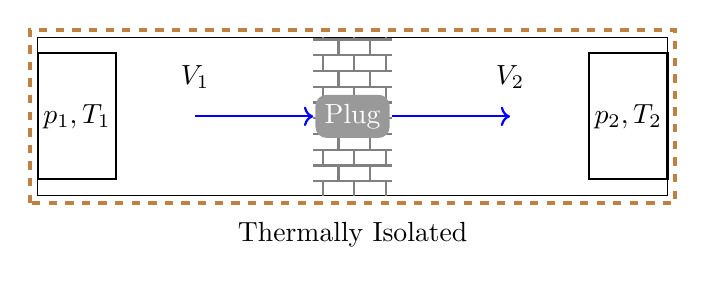
\begin{tikzpicture}
    % Walls
    \draw (-4, -1) rectangle (4, 1);
    % Porous Plug
    \fill [pattern=bricks, pattern color=gray] (-0.5, -1) rectangle (0.5, 1);
    \node at (0, 0) [white, fill=gray!80, text opacity=1, rounded corners] {Plug};
    % Pistons (conceptual)
    \draw [thick] (-4, -0.8) rectangle (-3, 0.8); \node at (-3.5, 0) {$p_1, T_1$};
    \draw [thick] (3, -0.8) rectangle (4, 0.8); \node at (3.5, 0) {$p_2, T_2$};
    % Flow Arrows
    \draw [->, blue, thick] (-2, 0) -- (-0.5, 0);
    \draw [->, blue, thick] (0.5, 0) -- (2, 0);
    % Labels
    \node at (-2, 0.5) {$V_1$};
    \node at (2, 0.5) {$V_2$};
    % Insulation
    \draw [line width=1.5pt, brown, dashed] (-4.1, -1.1) rectangle (4.1, 1.1);
    \node at (0, -1.5) {Thermally Isolated};
\end{tikzpicture}
\end{center}

Question: What is the final temperature $T_2$?

Analyze the process by considering a fixed amount (e.g., one mole) of gas passing through the plug.
Initial state: Gas occupies volume $V_1$ at $(p_1, T_1)$ with energy $E_1$.
Final state: Gas occupies volume $V_2$ at $(p_2, T_2)$ with energy $E_2$.

Work done during the process:
\begin{itemize}
    \item Work done *on* the gas on the left side to push it through the plug: $W_{on,1} = p_1 V_1$.
    \item Work done *by* the gas on the right side as it expands into volume $V_2$: $W_{by,2} = p_2 V_2$.
    \item Net work done *by* the gas: $W = W_{by,2} - W_{on,1} = p_2 V_2 - p_1 V_1$.
\end{itemize}
System is thermally isolated $\implies Q=0$.
First Law: $\Delta E = E_2 - E_1 = Q - W = 0 - (p_2 V_2 - p_1 V_1) = p_1 V_1 - p_2 V_2$.
Rearranging:
\[ E_1 + p_1 V_1 = E_2 + p_2 V_2 \]
Since Enthalpy is $H = E + pV$, this means:
\[ H_1 = H_2 \]
The Joule-Thomson process occurs at constant enthalpy. The final state $(T_2, p_2)$ is determined by $H(T_2, p_2) = H(T_1, p_1)$. (Compare with $E(T_2, V_2) = E(T_1, V_1)$ for free expansion).

\textbf{Ideal Gas Case:}
Enthalpy $H = E + pV$. For ideal gas, $E=E(T)$ and $pV=\nu \gasR T$.
So $H = E(T) + \nu \gasR T = H(T)$ only.
The condition $H(T_1) = H(T_2)$ implies $T_1 = T_2$ (assuming H is monotonic with T).
There is no temperature change for an ideal gas in a Joule-Thomson process.

\textbf{General Case:}
How does $T$ change with $p$ at constant $H$? We look at the Joule-Thomson coefficient $\mu_{JT}$:
\[ \mu_{JT} \equiv \left( \pderiv{T}{p} \right)_H \]
From $dH = (\partial H/\partial T)_p dT + (\partial H/\partial p)_T dp$, if $dH=0$:
\[ \left( \pderiv{T}{p} \right)_H = - \frac{(\partial H / \partial p)_T}{(\partial H / \partial T)_p} \]
We know $(\partial H / \partial T)_p = C_p$. We need $(\partial H / \partial p)_T$.
From $dH = T dS + V dp$:
Divide by $dp$ at constant $T$:
\[ \left( \pderiv{H}{p} \right)_T = T \left( \pderiv{S}{p} \right)_T + V \]
Use Maxwell relation $(\partial S / \partial p)_T = -(\partial V / \partial T)_p$:
\[ \left( \pderiv{H}{p} \right)_T = T \left[ - \left( \pderiv{V}{T} \right)_p \right] + V = V - T \left( \pderiv{V}{T} \right)_p \]
Substitute back into the expression for $\mu_{JT}$:
\[ \mu_{JT} = \left( \pderiv{T}{p} \right)_H = - \frac{1}{C_p} \left[ V - T \left( \pderiv{V}{T} \right)_p \right] = \frac{1}{C_p} \left[ T \left( \pderiv{V}{T} \right)_p - V \right] \]
Using the thermal expansion coefficient $\alpha_p = \frac{1}{V} (\partial V / \partial T)_p \implies (\partial V / \partial T)_p = V \alpha_p$.
\[ \mu_{JT} = \frac{1}{C_p} [T (V \alpha_p) - V] = \frac{V}{C_p} (T \alpha_p - 1) \]
The sign of $\mu_{JT}$ determines whether the gas cools ($\mu_{JT}>0$) or heats ($\mu_{JT}<0$) upon throttling (pressure drop, $dp<0$).
\begin{itemize}
    \item Cooling ($\Delta T < 0$ for $\Delta p < 0$) occurs if $\mu_{JT} > 0$, i.e., $T \alpha_p > 1$.
    \item Heating ($\Delta T > 0$ for $\Delta p < 0$) occurs if $\mu_{JT} < 0$, i.e., $T \alpha_p < 1$.
    \item $\mu_{JT}=0$ defines the "inversion curve" in the $(T,p)$ plane.
\end{itemize}
Ideal gas check: $\alpha_p = 1/T \implies T \alpha_p - 1 = 0 \implies \mu_{JT} = 0$.

\textbf{Entropy Change:}
From $dH = TdS + Vdp$, at constant $H$, $TdS = -Vdp \implies dS = -(V/T) dp$.
\[ \Delta S = S_2 - S_1 = \int_{p_1}^{p_2} \left( -\frac{V}{T} \right) dp \]
Since $p_2 < p_1$, $\Delta p = p_2 - p_1 < 0$. Also $V/T > 0$.
$\Delta S > 0$. The Joule-Thomson process is irreversible.

\textbf{Inversion Curve Diagram:}
Curves of constant enthalpy $H$ in the $(T,p)$ plane typically have the following qualitative form:

\begin{center}
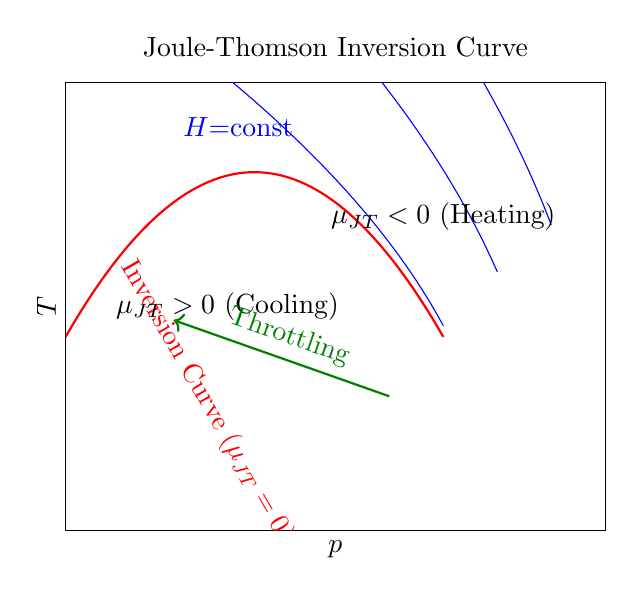
\begin{tikzpicture}
\begin{axis}[
    xlabel=$p$, ylabel=$T$,
    xmin=0, xmax=10, ymin=0, ymax=10,
    xtick=\empty, ytick=\empty,
    title={Joule-Thomson Inversion Curve}
]
% Constant H curves (schematic parabolas opening left)
\addplot [domain=1:9, samples=50, smooth, blue] {sqrt(40*(10-x))+0.5};
\addplot [domain=1:8, samples=50, smooth, blue] {sqrt(30*(9-x))+0.3};
\addplot [domain=1:7, samples=50, smooth, blue] {sqrt(20*(8-x))+0.1};
\node at (axis cs:2, 9) [anchor=west, blue] {$H$=const};

% Inversion curve (locus of maxima, schematic parabola opening down)
\addplot [domain=0:7, samples=50, smooth, thick, red] {-0.3*(x-3.5)^2+8} node [pos=0.2, anchor=west, rotate=-60] {Inversion Curve ($\mu_{JT}=0$)};

% Regions
\node at (axis cs:3, 5) {$\mu_{JT}>0$ (Cooling)};
\node at (axis cs:7, 7) {$\mu_{JT}<0$ (Heating)};

% Example process
\draw [->, thick, green!50!black] (axis cs:6, 3) -- (axis cs:2, 4.7) node[midway, above, sloped] {Throttling}; % Example crossing into cooling region
\end{axis}
\end{tikzpicture}
\end{center}
Inside the inversion curve (hatched region in source), $\mu_{JT}>0$, and throttling leads to cooling. Outside, $\mu_{JT}<0$, leading to heating. This process is used industrially to cool and liquefy gases by operating within the appropriate $(T,p)$ region.

\appendix
\section*{Appendix: $C_V$ for van der Waals Gas}

From general thermodynamics, we found $(\partial E/\partial V)_T = T(\partial p/\partial T)_V - p$.
Using the molar vdW equation $(p+a/v^2)(v-b)=RT$, we calculated $(\partial p/\partial T)_v = R/(v-b)$.
So, $(\partial \epsilon/\partial v)_T = T(\partial p/\partial T)_v - p = T(R/(v-b)) - p$.
Substituting $p = RT/(v-b) - a/v^2$:
\[ \left( \pderiv{\epsilon}{v} \right)_T = \frac{RT}{v-b} - \left( \frac{RT}{v-b} - \frac{a}{v^2} \right) = \frac{a}{v^2} \]
where $\epsilon = E/\nu$ is the molar internal energy.
Integrating with respect to $v$:
\[ \epsilon(T,v) = \int \frac{a}{v^2} dv = -\frac{a}{v} + f(T) \]
The molar energy is $\epsilon(T,v) = f(T) - a/v$. The total energy is $E(T,V) = \nu \epsilon = \nu f(T) - \nu^2 a / V$.
The molar heat capacity is:
\[ c_v = \left( \pderiv{\epsilon}{T} \right)_v = \pderiv{}{T} (f(T) - a/v) = f'(T) \]
So $c_v$ depends only on $T$.
To find $f(T)$, consider the dilute limit $v \to \infty$. In this limit, the vdW gas behaves like an ideal gas.
$\epsilon(T, v \to \infty) = f(T)$. This must equal the molar energy of the corresponding ideal gas, $\epsilon^{ideal}(T)$.
Let $c_v^{ideal}(T)$ be the molar specific heat of the ideal gas. Then $\epsilon^{ideal}(T) = \int c_v^{ideal}(T) dT + \text{const}$.
So $f(T) = \epsilon^{ideal}(T)$.
Then $c_v^{vdW}(T) = f'(T) = \deriv{\epsilon^{ideal}}{T} = c_v^{ideal}(T)$.
Conclusion: The molar heat capacity $c_v$ for a van der Waals gas is the same function of $T$ as for the corresponding ideal gas (e.g., $\frac{3}{2}R$ for monatomic). It does not depend on volume $v$.

\end{document}